\clearpage
\maketitlesupplementary
\setcounter{page}{1}
\onecolumn

\noindent\makebox[0pt][l]{%
  \begin{minipage}{\textwidth}
    \section{Colour Hists + HOG + Random Forest}
    \label{sec:suppl-rf-confusion}

    The following matrices correspond to the classification performance of the Random Forest method.

    The first matrix shows the species codes for the 20 most commonly confused species pairs by the model (30+ total species) \cref{fig:top20_confused}.

    \centering

    \begin{minipage}{\linewidth}
      \centering
      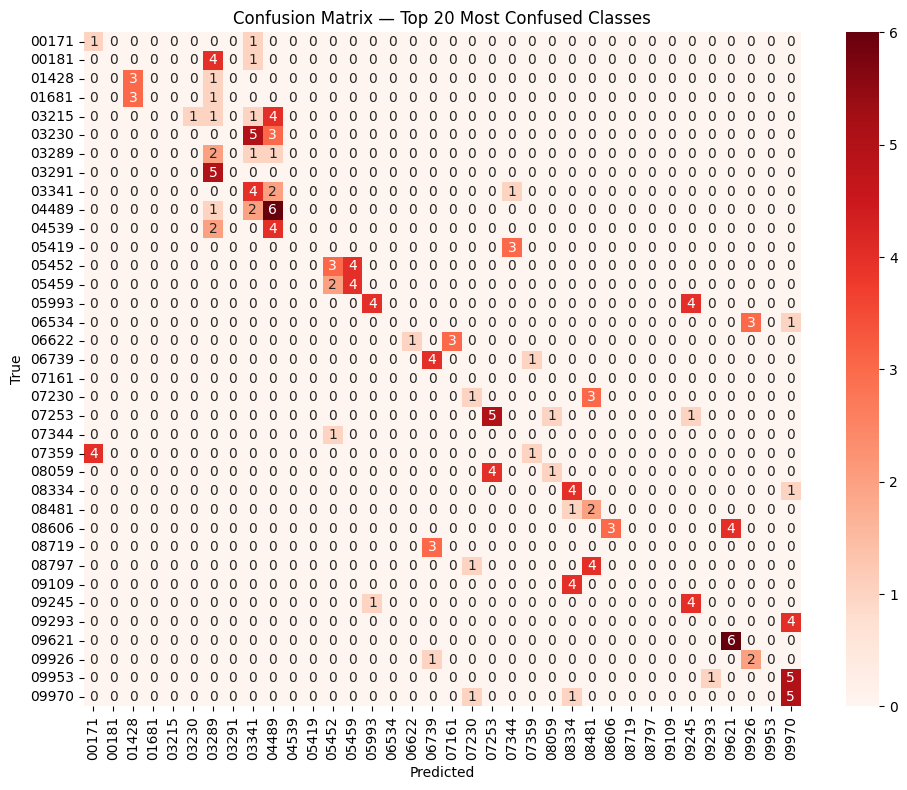
\includegraphics[width=0.7\linewidth]
      {../comprehensive_method_development/traditional_methods/traditional_rf/20_most_confused.png}
    \end{minipage}

    \captionsetup{hypcap=false}
    \captionof{figure}{Confusion matrix of the top 20 most confused class pairs.}
    \label{fig:top20_confused}

    The second matrix shows the classification accuracy on a phylum level \cref{fig:cm_phylum_level}.

    \begin{minipage}{\linewidth}
      \centering
      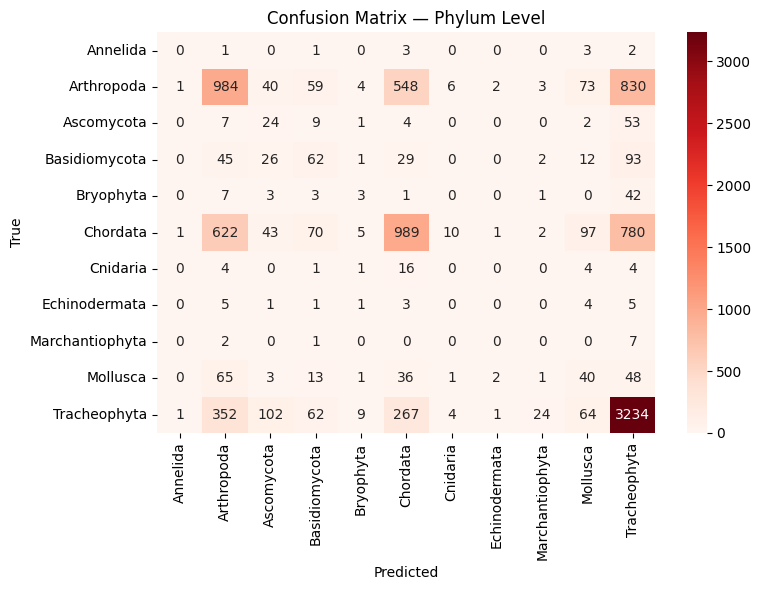
\includegraphics[width=0.6\linewidth]
      {../comprehensive_method_development/traditional_methods/traditional_rf/cm_phylum_level.png}
    \end{minipage}

    \captionof{figure}{Confusion matrix at the phylum level.}
    \label{fig:cm_phylum_level}

  \end{minipage}%
}

\par
\clearpage

\noindent\makebox[0pt][l]{%
  \begin{minipage}{\textwidth}
    \section{BoVW--RootSIFT--SVM confusion matrices}
    \label{sec:suppl-svm-confusion}

    The following confusion matrices show the classification performance of
    the improved BoVW--RootSIFT--SVM representation. The first matrix includes
    all 1{,}000 species, while the second focuses on the most-confused species.

    \centering

    \begin{minipage}{0.48\linewidth}
      \centering
      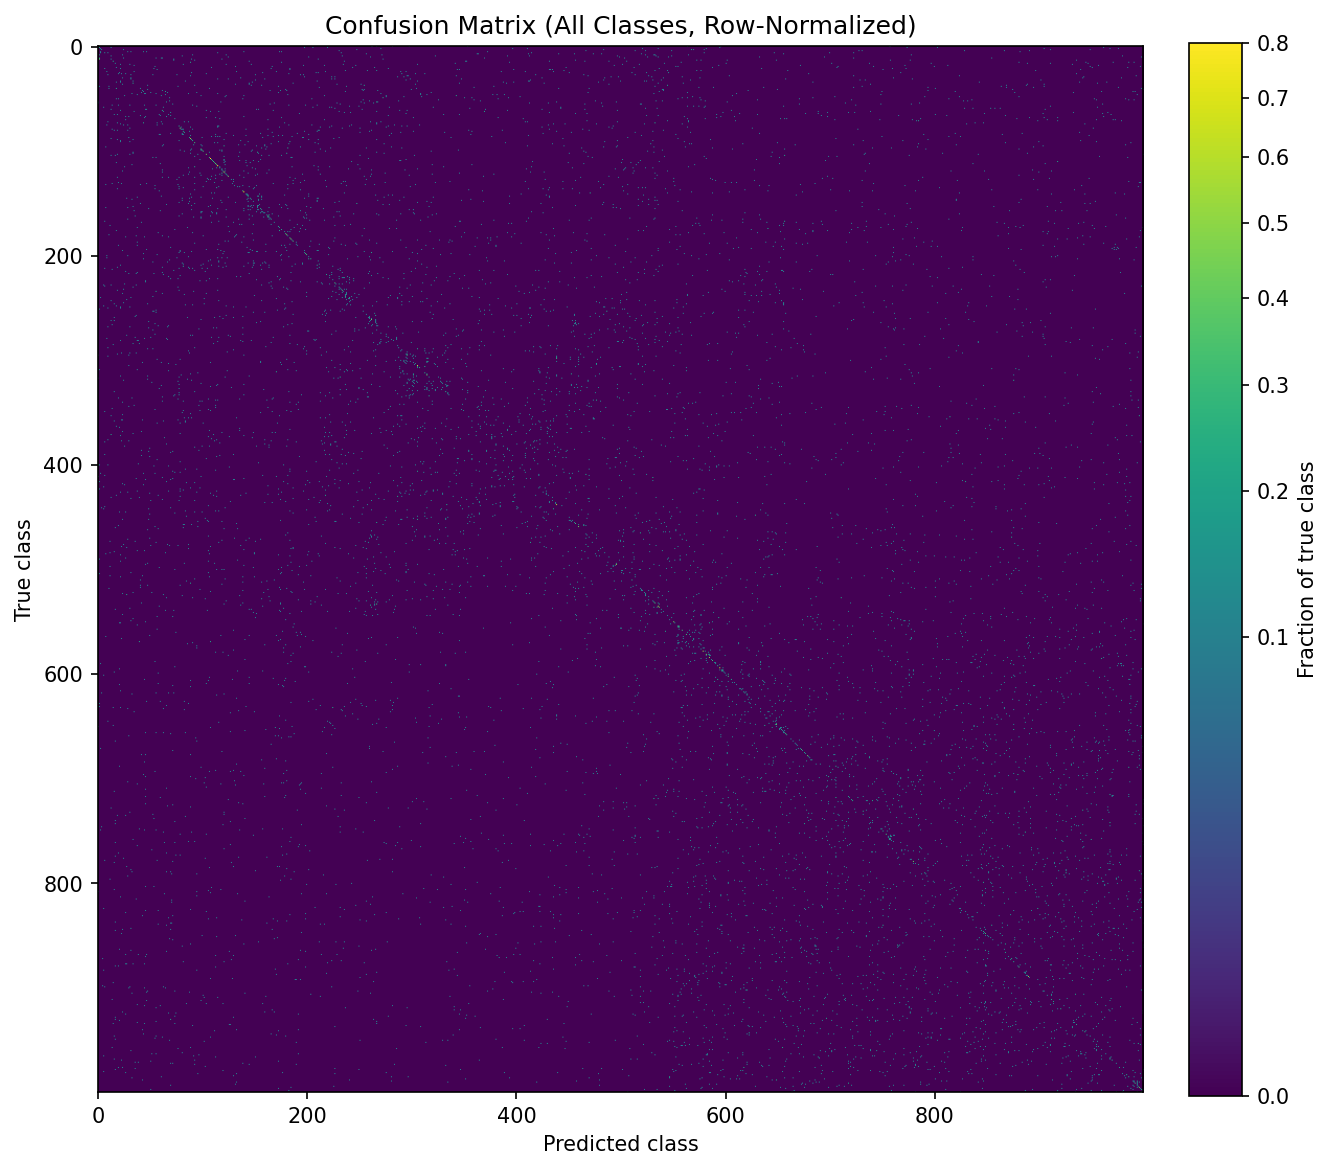
\includegraphics[width=\linewidth]
      {../comprehensive_method_development/traditional_methods/traditional_bovw/traditional_bovw_results/final_confusion_matrix.png}

      {\small (a) All 1{,}000 species\par}
    \end{minipage}
    \hfill
    \begin{minipage}{0.48\linewidth}
      \centering
      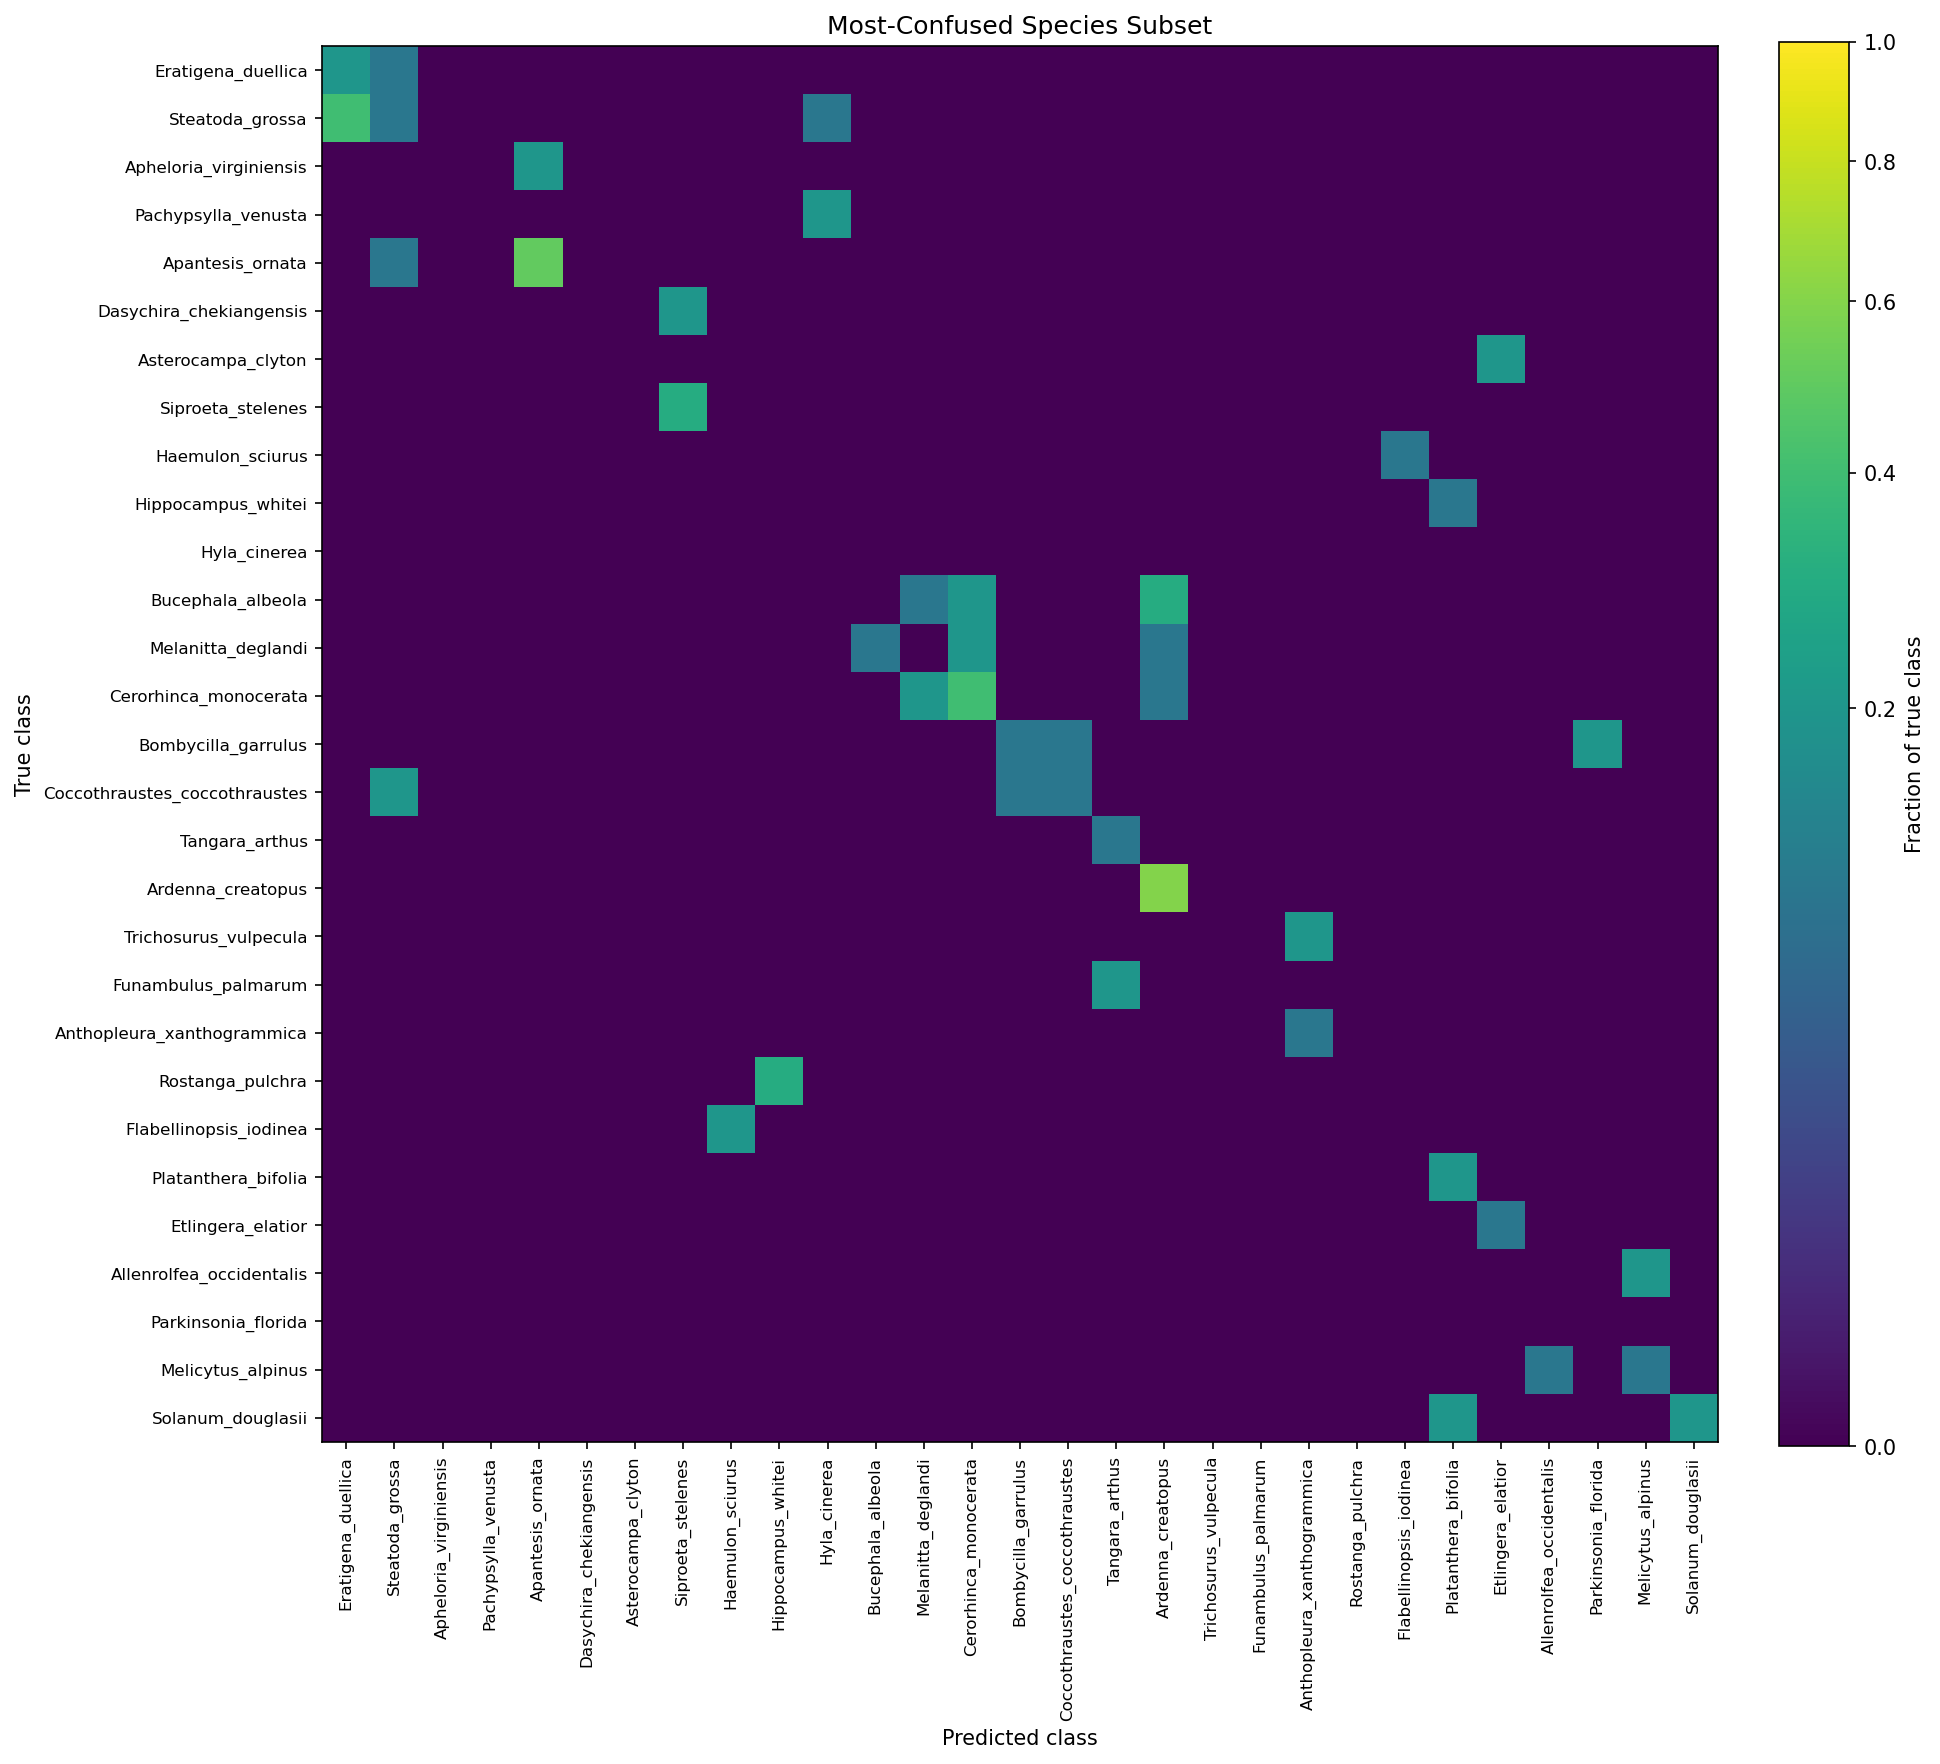
\includegraphics[width=\linewidth]
      {../comprehensive_method_development/traditional_methods/traditional_bovw/traditional_bovw_results/final_confusion_matrix_subset.png}

      {\small (b) Most-confused species\par}
    \end{minipage}

    \captionsetup{hypcap=false}
    \captionof{figure}{
      Confusion matrices for the improved BoVW--RootSIFT--SVM representation.
      (a) Row-normalised confusion matrix over all 1{,}000 species. The faint
      diagonal against a diffuse error background reflects the low but
      above-chance accuracy of a hand-crafted pipeline on a 1{,}000-way
      fine-grained classification task.
      (b) Confusion matrix restricted to the most-confused species. The
      strongest off-diagonal cells occur between visually and taxonomically
      similar species, including cobweb spiders
      \textit{Eratigena}/\textit{Steatoda} and dark-plumaged seabirds and
      waterfowl
      \textit{Bucephala}/\textit{Melanitta}/\textit{Cerorhinca}.
    }
    \label{fig:suppl-svm-confusion}
    \label{fig:suppl-svm-confusion-full}
    \label{fig:suppl-svm-confusion-subset}

  \end{minipage}%
}

\par
\clearpage

\noindent\makebox[0pt][l]{%
  \begin{minipage}{\textwidth}
    \section{EfficientNet V2 training hyperparameters}
    \label{sec:suppl-efficientnetv2-hyperparams}

    \cref{tab:efficientnetv2-hyperparams} lists the training hyperparameter settings for the EfficientNet V2 pretrained and from-scratch regimes described in \cref{sec:dl-efficientnetv2}.

    \begin{center}
      \captionsetup{hypcap=false}
      \captionof{table}{EfficientNet V2-S training hyperparameters for pretrained and from-scratch runs. Settings marked ``ablated'' are varied across the six experiments in \cref{tab:efficientnetv2-results}. Rows marked \emph{(aug.)} are data augmentation components.}
      \label{tab:efficientnetv2-hyperparams}
      \small
      \begin{tabular}{@{}lll@{}}
        \toprule
        Setting                      & Pretrained                         & From scratch                       \\
        \midrule
        Optimizer                    & AdamW                              & AdamW                              \\
        LR schedule                  & Cosine decay + linear warmup       & Cosine decay + linear warmup       \\
        Initial learning rate        & $5\times10^{-5}$                   & $1\times10^{-3}$                   \\
        Weight decay                 & 0.05                               & 0.05                               \\
        Stochastic depth             & 0.2 (fixed)                        & 0.2 (fixed)                        \\
        Classifier dropout           & 0.2                                & 0.2                                \\
        Augmentation level (ablated) & None / Crop / Crop+Flip / Full     & None / Full                        \\
        RandomResizedCrop (aug.)     & scale $=(0.7, 1.0)$                & scale $=(0.7, 1.0)$                \\
        HorizontalFlip (aug.)        & $p=0.5$                            & $p=0.5$                            \\
        ColorJitter (aug.)           & b/c/s $=0.2$, hue $=0.05$, $p=0.5$ & b/c/s $=0.2$, hue $=0.05$, $p=0.5$ \\
        Warmup steps                 & 1,000 (fixed)                      & 1,000 (fixed)                      \\
        Early-stopping patience      & 5                                  & 5                                  \\
        Early-stopping threshold     & 0.0                                & 0.0                                \\
        Batch size                   & 128 (effective)                    & 128 (effective)                    \\
        Label smoothing              & 0.1                                & 0.1                                \\
        \bottomrule
      \end{tabular}
    \end{center}
  \end{minipage}%
}
\par

\clearpage
\noindent\makebox[0pt][l]{%
  \begin{minipage}{\textwidth}
    \section{EfficientNet V2 training curves}
    \label{sec:suppl-efficientnetv2-curves}

    \cref{fig:suppl-efficientnetv2-loss} shows training and validation loss for all six runs in \cref{tab:efficientnetv2-results}.

    \centering
    \begin{minipage}{0.48\linewidth}
      \centering
      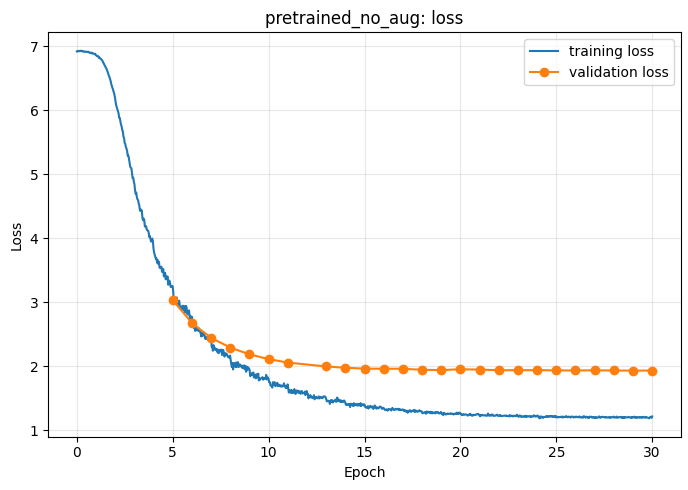
\includegraphics[width=\linewidth]{image/deep_learning_based_methods/efficientnetv2/loss_curve_a_pretrained_no_aug.png}
      {\small (a) Exp.\ A (pretrained, None)\par}
    \end{minipage}\hfill
    \begin{minipage}{0.48\linewidth}
      \centering
      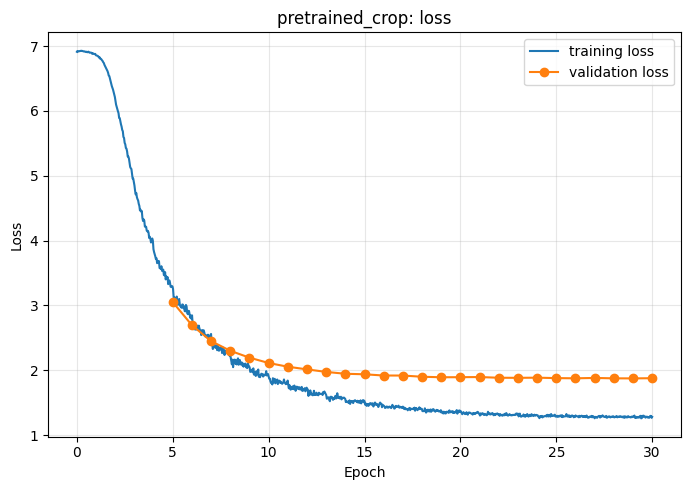
\includegraphics[width=\linewidth]{image/deep_learning_based_methods/efficientnetv2/loss_curve_d_pretrained_crop.png}
      {\small (b) Exp.\ B (pretrained, Crop)\par}
    \end{minipage}
    \par\vspace{0.4em}
    \begin{minipage}{0.48\linewidth}
      \centering
      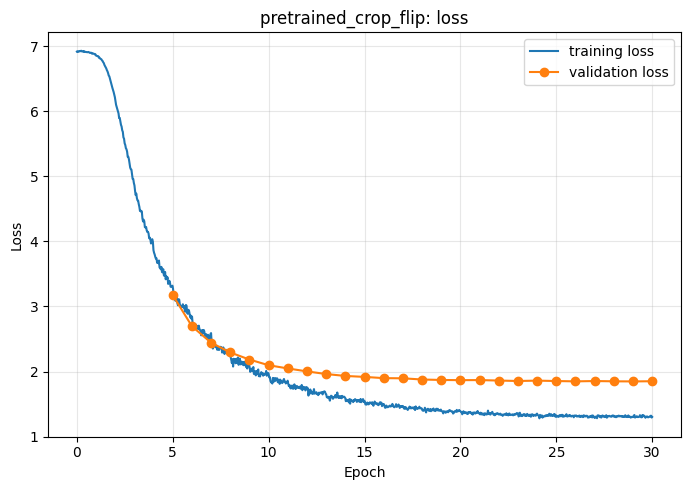
\includegraphics[width=\linewidth]{image/deep_learning_based_methods/efficientnetv2/loss_curve_e_pretrained_cropflip.png}
      {\small (c) Exp.\ C (pretrained, Crop+Flip)\par}
    \end{minipage}\hfill
    \begin{minipage}{0.48\linewidth}
      \centering
      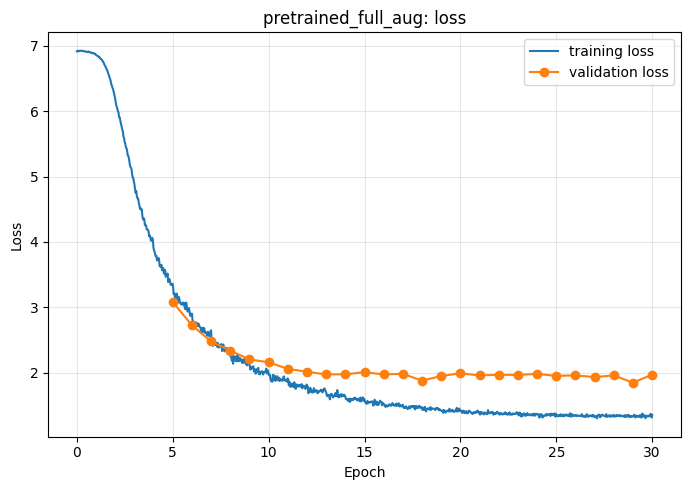
\includegraphics[width=\linewidth]{image/deep_learning_based_methods/efficientnetv2/loss_curve_b_pretrained_aug.png}
      {\small (d) Exp.\ D (pretrained, Full)\par}
    \end{minipage}
    \par\vspace{0.4em}
    \begin{minipage}{0.48\linewidth}
      \centering
      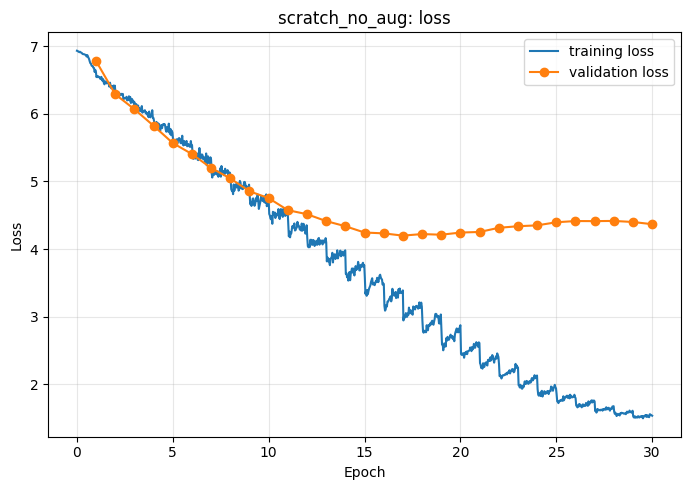
\includegraphics[width=\linewidth]{image/deep_learning_based_methods/efficientnetv2/loss_curve_c_scratch_no_aug.png}
      {\small (e) Exp.\ E (scratch, None)\par}
    \end{minipage}\hfill
    \begin{minipage}{0.48\linewidth}
      \centering
      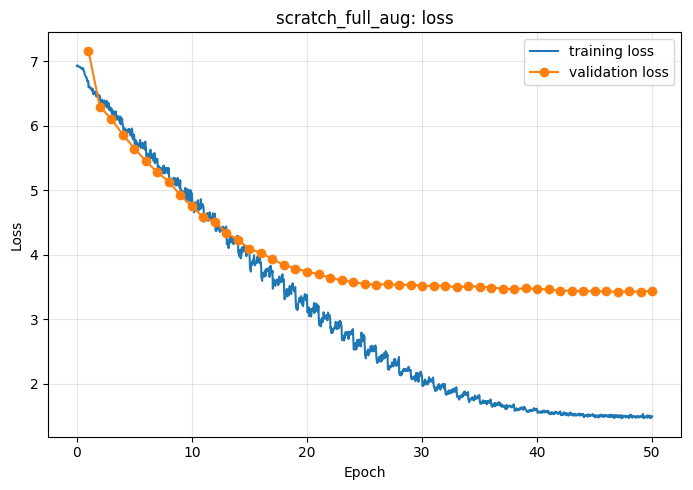
\includegraphics[width=\linewidth]{image/deep_learning_based_methods/efficientnetv2/loss_curve_d_scratch_aug.png}
      {\small (f) Exp.\ F (scratch, Full)\par}
    \end{minipage}
    \captionsetup{hypcap=false}
    \captionof{figure}{EfficientNet V2 training and validation loss curves for experiments A--F from \cref{tab:efficientnetv2-results}.}
    \label{fig:suppl-efficientnetv2-loss}
  \end{minipage}%
}
\par

\clearpage
\noindent\makebox[0pt][l]{%
  \begin{minipage}{\textwidth}
    \section{EfficientNet V2 phylum-level confusion matrices}
    \label{sec:suppl-efficientnetv2-phylum}

    \cref{fig:suppl-efficientnetv2-phylum} shows phylum-aggregated predictions for experiment C from \cref{tab:efficientnetv2-results}, corresponding to the analysis in \cref{sec:dl-efficientnetv2-error-analysis}.

    \centering
    \begin{minipage}{0.48\linewidth}
      \centering
      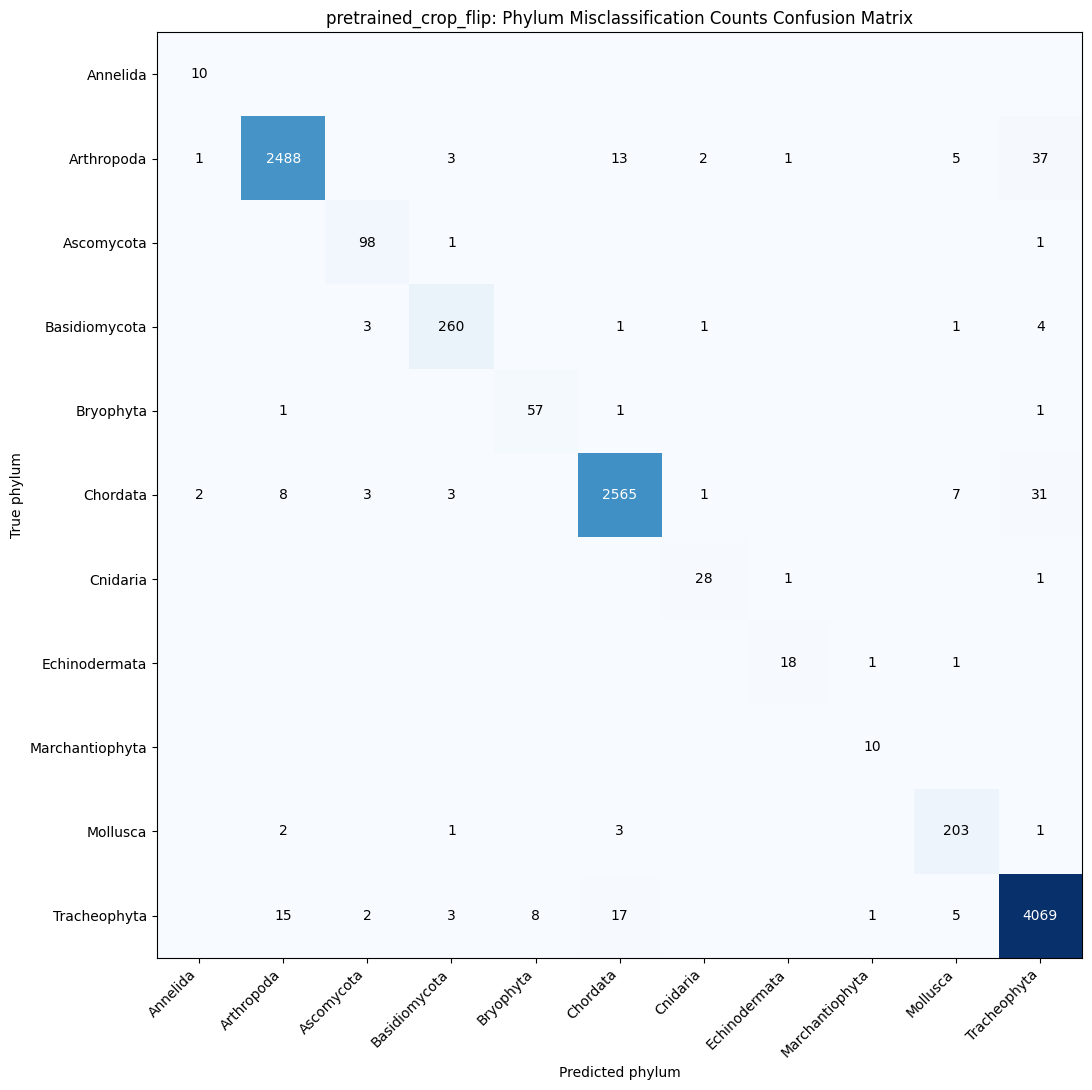
\includegraphics[width=\linewidth]{image/deep_learning_based_methods/efficientnetv2/phylum_level_confusion_matrix_counts.png}
      {\small (a) Counts\par}
    \end{minipage}\hfill
    \begin{minipage}{0.48\linewidth}
      \centering
      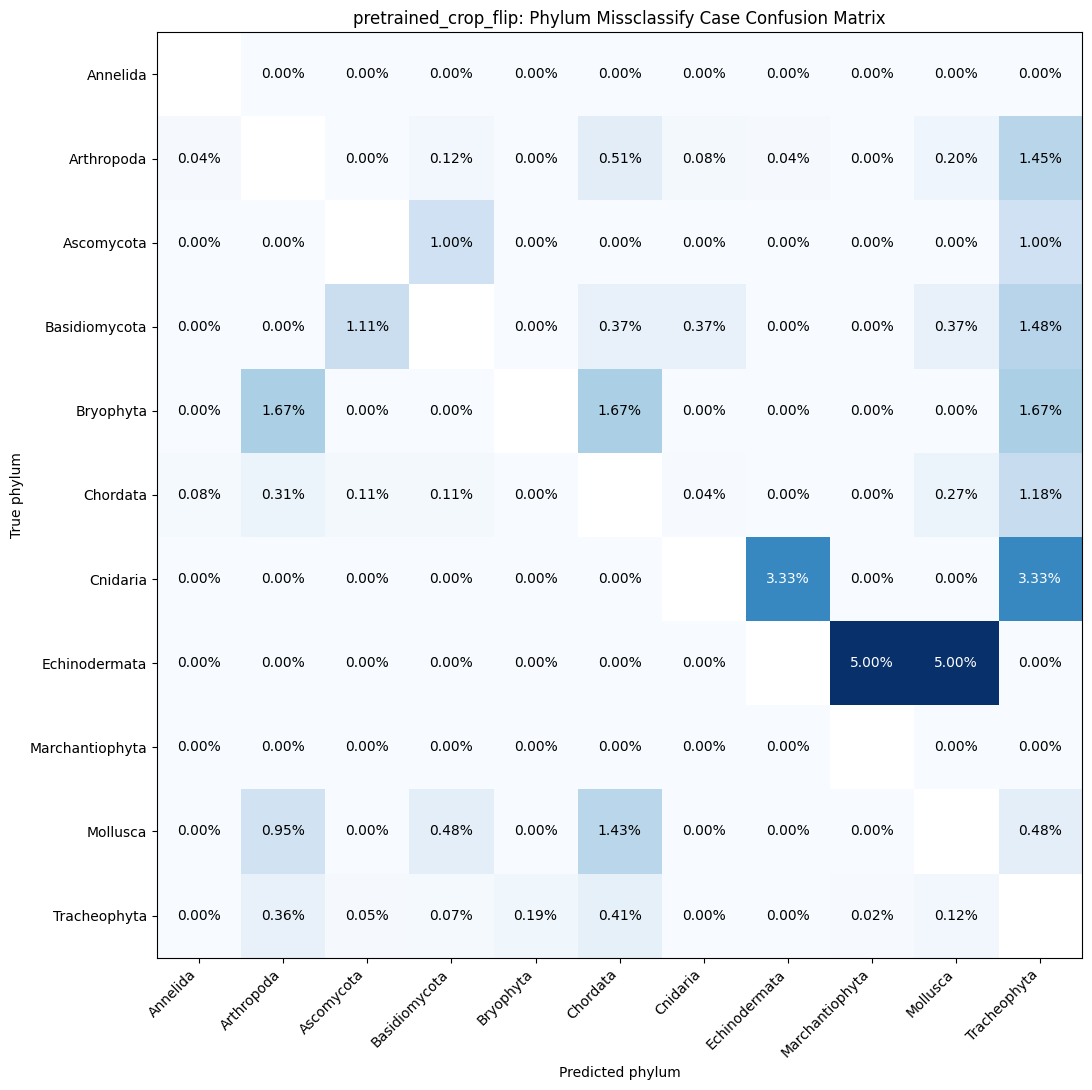
\includegraphics[width=\linewidth]{image/deep_learning_based_methods/efficientnetv2/phylum_level_confusion_matrix_percentage.png}
      {\small (b) Row-normalized misclassification rates\par}
    \end{minipage}
    \captionsetup{hypcap=false}
    \captionof{figure}{Phylum-level confusion matrices for EfficientNet V2 experiment C. (a) Absolute counts including correct predictions on the diagonal. (b) Row-normalized off-diagonal misclassification rates.}
    \label{fig:suppl-efficientnetv2-phylum}
  \end{minipage}%
}
\par
\clearpage
\noindent\makebox[0pt][l]{%
  \begin{minipage}{\textwidth}
    \section{ConvNeXt V2 training hyperparameters}
    \label{sec:suppl-convnextv2-hyperparams}

    \cref{tab:convnextv2-hyperparams} lists the full training hyperparameter settings for the ConvNeXt V2 pretrained and from-scratch regimes described in \cref{sec:dl-convnextv2}.

    \begin{center}
      \captionsetup{hypcap=false}
      \captionof{table}{ConvNeXt V2 training hyperparameters for pretrained and from-scratch runs. Settings marked ``ablated'' are varied across the $9$ experiments in \cref{tab:main-results}. Rows marked \emph{(aug.)} are data augmentation components; \emph{+CD}/\emph{+Mix} indicate the ablation tier introducing each.}
      \label{tab:convnextv2-hyperparams}
      \small
      \begin{tabular}{@{}lll@{}}
        \toprule
        Setting                      & Pretrained                         & From scratch                                 \\
        \midrule
        Optimizer                    & AdamW                              & AdamW                                        \\
        LR schedule                  & Cosine decay + linear warmup       & Cosine decay + linear warmup                 \\
        Initial learning rate        & $5\times10^{-5}$                   & $1\times10^{-3}$                             \\
        Weight decay                 & 0.05                               & 0.05                                         \\
        DropPath                     & 0 (fixed)                          & 0 / 0.1 (ablated)                            \\
        Augmentation level (ablated) & None / Basic                       & None / Basic / Basic+CD / Basic+CD+Mix       \\
        RandomResizedCrop (aug.)     & scale $=(0.7, 1.0)$                & scale $=(0.7, 1.0)$                          \\
        HorizontalFlip (aug.)        & $p=0.5$                            & $p=0.5$                                      \\
        ColorJitter (aug.)           & b/c/s $=0.2$, hue $=0.05$, $p=0.5$ & b/c/s $=0.2$, hue $=0.05$, $p=0.5$           \\
        CoarseDropout (aug., +CD)    & --                                 & holes $=(3,8)$, size $=(0.05,0.15)$, $p=0.5$ \\
        CutMix/MixUp (aug., +Mix)    & --                                 & batch-level                                  \\
        Warmup steps                 & 1000 (fixed)                       & 1000 / 10000 / 30000 (ablated)               \\
        Early-stopping patience      & 5                                  & 5                                            \\
        Early-stopping threshold     & 0.0                                & 0.0                                          \\
        Batch size                   & 128                                & 128                                          \\
        Label smoothing              & 0.1                                & 0.1                                          \\
        \bottomrule
      \end{tabular}
    \end{center}
  \end{minipage}%
}
\par

\clearpage
\noindent\makebox[0pt][l]{%
  \begin{minipage}{\textwidth}
    \section{ConvNeXt V2 training curves}
    \label{sec:suppl-convnextv2-curves}

    \cref{fig:suppl-convnextv2-loss} shows training and validation loss versus epoch for a curated subset of the A--I ablation in \cref{tab:main-results}: the best pretrained run (B), the scratch baseline without augmentation (C), the best from-scratch run (H), and the over-long warmup failure case (I).

    \centering
    \begin{minipage}{0.48\linewidth}
      \centering
      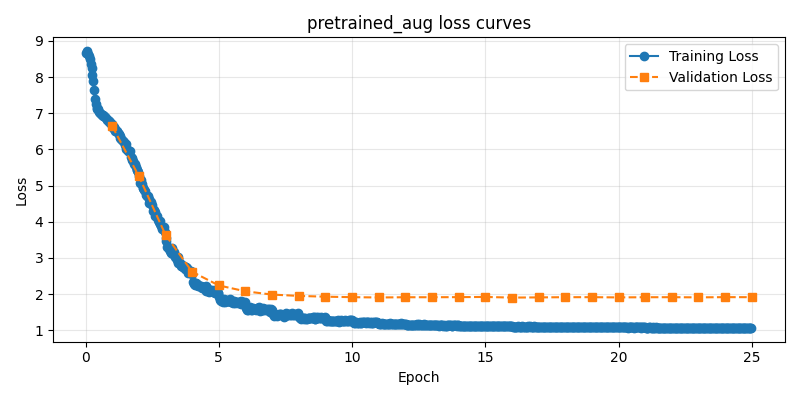
\includegraphics[width=\linewidth]{image/deep_learning_based_methods/convnextv2/loss_curve_b_pretrained_aug.png}
      {\small (a) Exp.\ B (pretrained, Basic)\par}
    \end{minipage}\hfill
    \begin{minipage}{0.48\linewidth}
      \centering
      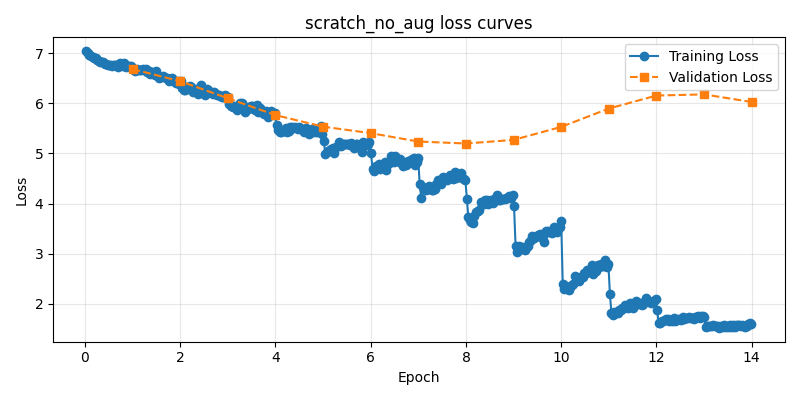
\includegraphics[width=\linewidth]{image/deep_learning_based_methods/convnextv2/loss_curve_c_scratch_no_aug.png}
      {\small (b) Exp.\ C (scratch, None)\par}
    \end{minipage}
    \par\vspace{0.4em}
    \begin{minipage}{0.48\linewidth}
      \centering
      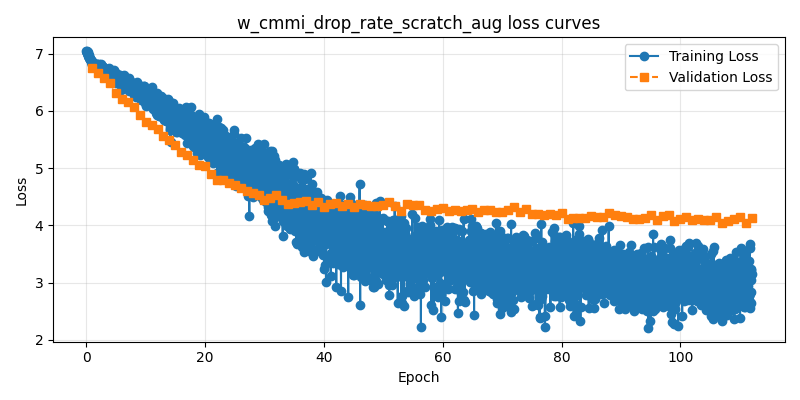
\includegraphics[width=\linewidth]{image/deep_learning_based_methods/convnextv2/loss_curve_h_w_cmmi_drop_rate_scratch_aug.png}
      {\small (c) Exp.\ H (scratch, Basic+CD+Mix, 10k warmup)\par}
    \end{minipage}\hfill
    \begin{minipage}{0.48\linewidth}
      \centering
      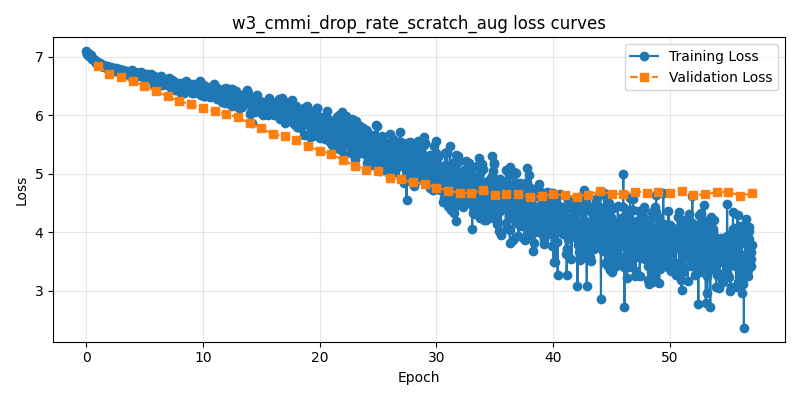
\includegraphics[width=\linewidth]{image/deep_learning_based_methods/convnextv2/loss_curve_i_w3_cmmi_drop_rate_scratch_aug.png}
      {\small (d) Exp.\ I (scratch, Basic+CD+Mix, 30k warmup)\par}
    \end{minipage}
    \captionsetup{hypcap=false}
    \captionof{figure}{ConvNeXt V2 training (solid) and validation (dashed) loss curves for experiments B, C, H, and I from \cref{tab:main-results}.}
    \label{fig:suppl-convnextv2-loss}
  \end{minipage}%
}
\par

\clearpage
\noindent\makebox[0pt][l]{%
  \begin{minipage}{\textwidth}
    \section{ConvNeXt V2 phylum-level confusion matrices}
    \label{sec:suppl-convnextv2-phylum}

    \cref{fig:suppl-convnextv2-phylum} shows phylum-aggregated predictions for experiment B from \cref{tab:main-results}, corresponding to the analysis in \cref{sec:dl-convnextv2}.

    \centering
    \begin{minipage}{0.48\linewidth}
      \centering
      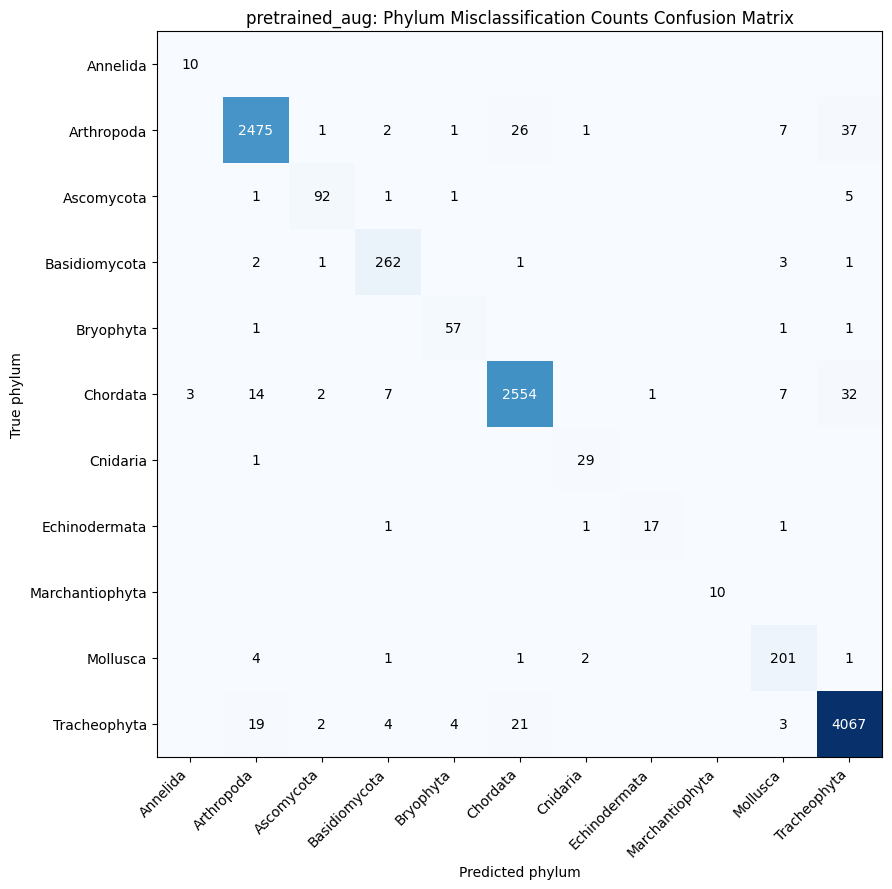
\includegraphics[width=\linewidth]{image/deep_learning_based_methods/convnextv2/phylum_level_confusion_matrix_number.png}
      {\small (a) Counts\par}
    \end{minipage}\hfill
    \begin{minipage}{0.48\linewidth}
      \centering
      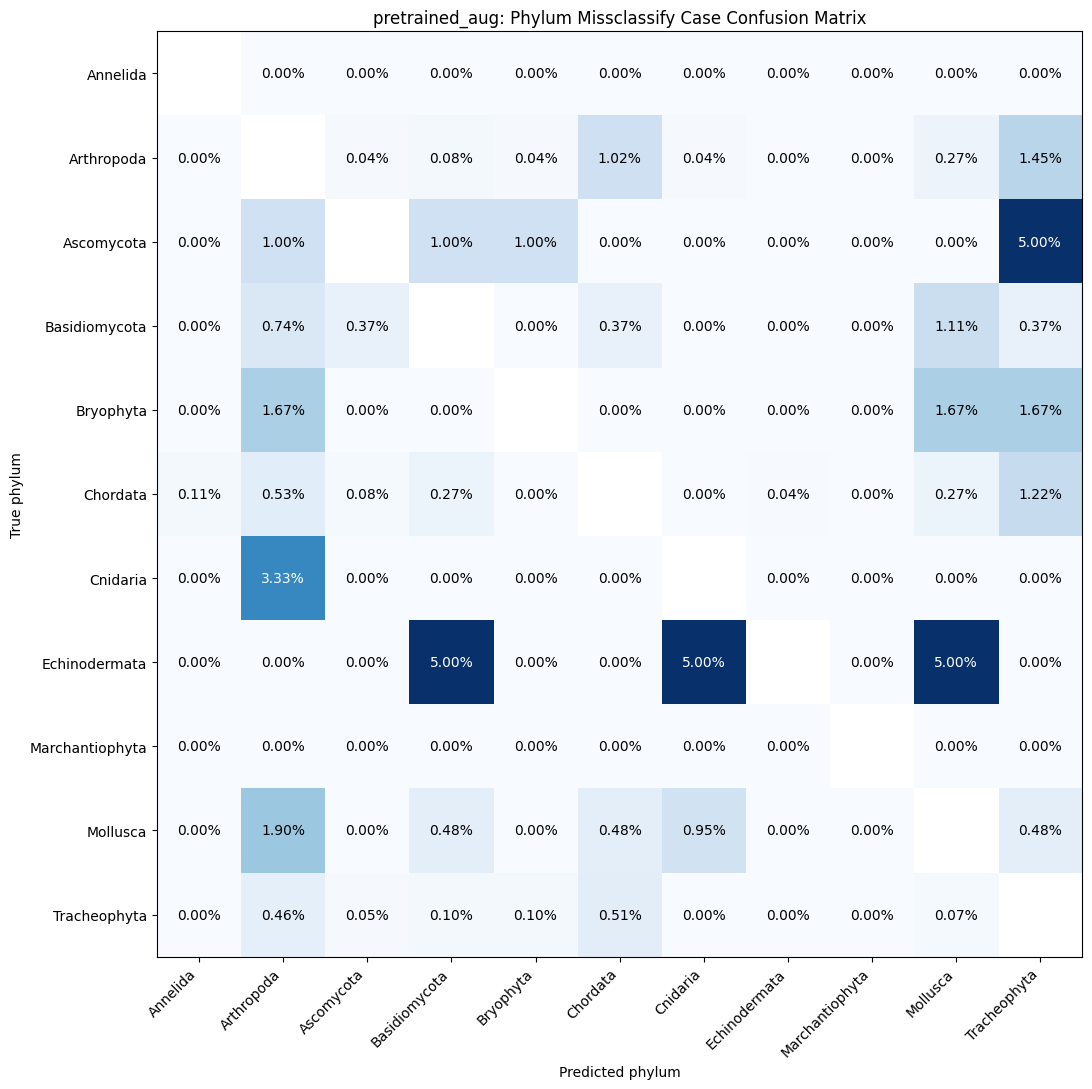
\includegraphics[width=\linewidth]{image/deep_learning_based_methods/convnextv2/phylum_level_confusion_matrix_percentage.png}
      {\small (b) Row-normalized misclassification rates\par}
    \end{minipage}
    \captionsetup{hypcap=false}
    \captionof{figure}{Phylum-level confusion matrices for ConvNeXt V2 experiment B. (a) Absolute counts including correct predictions on the diagonal. (b) Row-normalized off-diagonal misclassification rates.}
    \label{fig:suppl-convnextv2-phylum}
  \end{minipage}%
}
\par

\clearpage
\noindent\makebox[0pt][l]{%
  \begin{minipage}{\textwidth}
    \section{Grad-CAM Confusable Species Pairs}
    \label{sec:suppl-gradcam-confusable}

    \cref{fig:suppl-gradcam-confusable} illustrates Grad-CAM visual explanations across three confusable genus pairs from distinct biological classes: Spiders (\textit{Steatoda}), Bumblebees (\textit{Bombus}), and Mint Moths (\textit{Pyrausta}), supplementing the analysis in \cref{sec:part3-confusable}.

    \centering
    \begin{minipage}{0.48\linewidth}
      \centering
      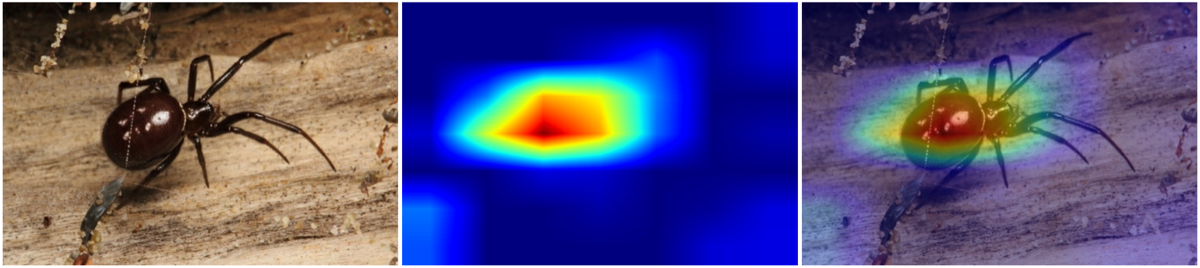
\includegraphics[width=\linewidth]{image/grad_cam/gradcam_confusable_steatoda_1.png}
      {\small (a) \textit{Steatoda capensis} (True: \textit{S. capensis}, Pred: \textit{S. capensis}, Prob: 0.3292)\par}
    \end{minipage}\hfill
    \begin{minipage}{0.48\linewidth}
      \centering
      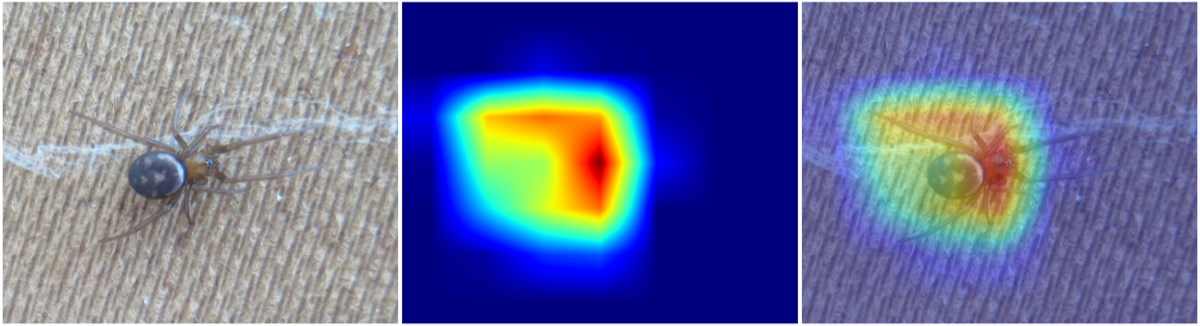
\includegraphics[width=\linewidth]{image/grad_cam/gradcam_confusable_steatoda_2.png}
      {\small (b) \textit{Steatoda grossa} (True: \textit{S. grossa}, Pred: \textit{S. grossa}, Prob: 0.3977)\par}
    \end{minipage}
    \par\vspace{0.4em}
    \begin{minipage}{0.48\linewidth}
      \centering
      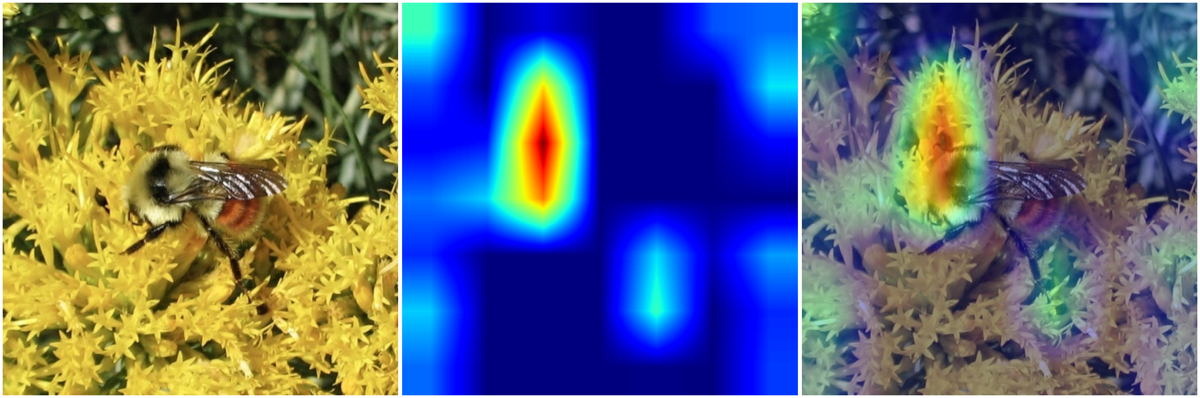
\includegraphics[width=\linewidth]{image/grad_cam/gradcam_confusable_bombus_1.png}
      {\small (c) \textit{Bombus huntii} (True: \textit{B. huntii}, Pred: \textit{B. huntii}, Prob: 0.2010)\par}
    \end{minipage}\hfill
    \begin{minipage}{0.48\linewidth}
      \centering
      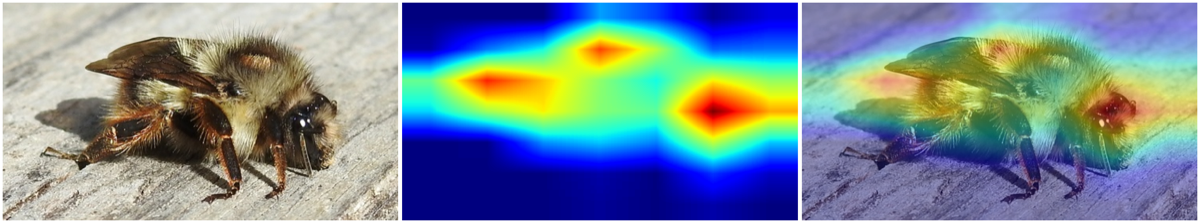
\includegraphics[width=\linewidth]{image/grad_cam/gradcam_confusable_bombus_2.png}
      {\small (d) \textit{Bombus mixtus} (True: \textit{B. mixtus}, Pred: \textit{B. mixtus}, Prob: 0.8920)\par}
    \end{minipage}
    \par\vspace{0.4em}
    \begin{minipage}{0.48\linewidth}
      \centering
      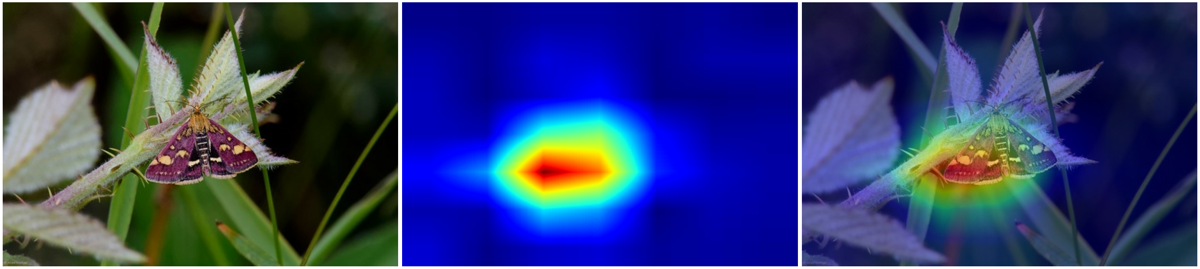
\includegraphics[width=\linewidth]{image/grad_cam/gradcam_confusable_pyrausta_1.png}
      {\small (e) \textit{Pyrausta purpuralis} (True: \textit{P. purpuralis}, Pred: \textit{P. purpuralis}, Prob: 0.3538)\par}
    \end{minipage}\hfill
    \begin{minipage}{0.48\linewidth}
      \centering
      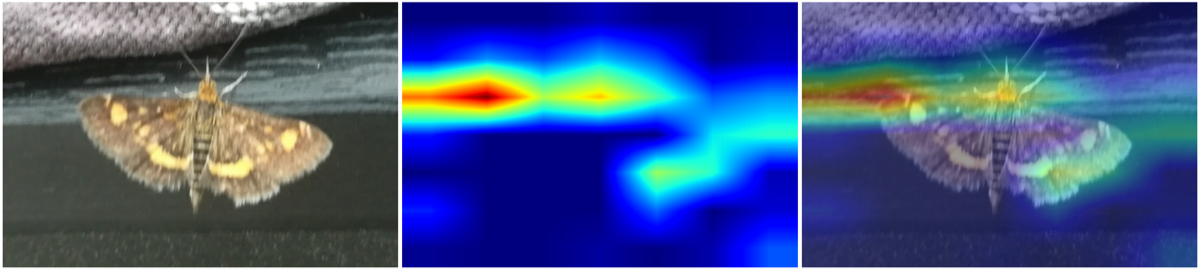
\includegraphics[width=\linewidth]{image/grad_cam/gradcam_confusable_pyrausta_2.png}
      {\small (f) \textit{Pyrausta aurata} (True: \textit{P. aurata}, Pred: \textit{P. aurata}, Prob: 0.4671)\par}
    \end{minipage}
    \captionsetup{hypcap=false}
    \captionof{figure}{\textbf{Grad-CAM comparison across three confusable genus pairs.} Top row: Genus \textit{Steatoda} (Cobweb Spiders). Middle row: Genus \textit{Bombus} (Bumblebees). Bottom row: Genus \textit{Pyrausta} (Mint Moths).}
    \label{fig:suppl-gradcam-confusable}
    \label{fig:gradcam_confusable_pairs}
    \label{fig:gradcam_steatoda}
    \label{fig:gradcam_bombus}
    \label{fig:gradcam_pyrausta}
  \end{minipage}%
}
\par